\section{Name Prefix Table}
\label{sec:npt}

\begin{figure}[!h]
  \center
  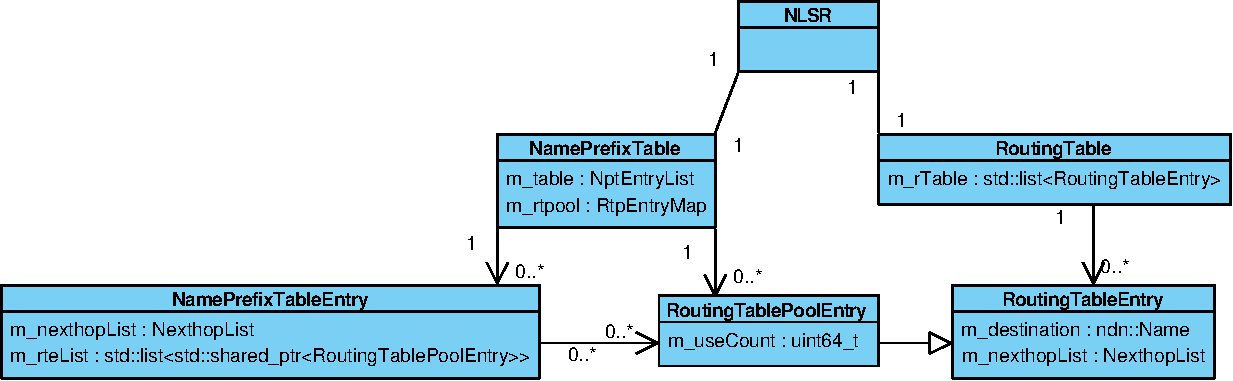
\includegraphics[width=0.8\linewidth]{npt.pdf}
  \begin{caption}
    A diagram of the NPT and Routing Table.

    \begin{footnotesize}
      The ``wire'' arrows represent references (i.e. ``x has y''),
      whereas the ``solid'' arrows represent inheritance (i.e. ``y subclasses x''). \\
      The quantification (e.g. 0..*) is standard UML.
    \end{footnotesize}
  \end{caption}
  \label{fig:npt-class-diagram}
\end{figure}

The Name Prefix Table (NPT) is used by NLSR to maintain a list of all known name prefixes advertised by other routers, including router names.
The NPT maintains a collection of NPT entries, where each entry represents a name prefix and all of its associated routing table entries.
Additionally, to optimize the storage and association of the routing table entries, the NPT also maintains a collection of duplicated routing table entries, called routing table pool entries, which have an additional use count attribute.
The NPT entries keep shared pointers to the appropriate routing table pool entries.
If a name prefix is advertised by multiple routers, the name prefix will be represented by only one Name Prefix Table Entry, but will have multiple routing table pool entries  which correspond with each origin router.

If a Name LSA exists with some advertised name prefix, then that prefix must have an entry in the NPT. So, if two routers advertise the same name prefix, i.e. their name LSAs contain a common name prefix, even if one router withdraws that common name prefix, the entry must remain in the NPT, because the other router still advertises it.

If any type of LSA for a remote router exists in the LSDB, the remote router's name prefix must be in the NPT.
An NPT Entry for a router name can only be removed when there are no more LSAs in the LSDB from the origin router. Note, even if some NPT entry nas no next hops, it will \emph{not} be removed from the NPT; it may later become possible to route to this prefix. These prefixes will be removed from the FIB, however.

\subsection{Adding an NPT Entry}
\label{sec:npt-add}
The \texttt{NamePrefixTable::addEntry()} method is the public
interface for name prefixes to be added to the NPT.
The name prefix as well as the router's prefix which originates the
name prefix are passed as parameters to the method.

If the name prefix is new, there will be no NPT entry for it, so one
will be created. If the name prefix is not new, the existing entry
will be updated, so the existing entry will also store this new origin
router's prefix, too. If after updating, the NPT entry has any next
hops, which are associated to each of the origin router prefixes, the
NPT will update the FIB to include that prefix and its next hops. The
next hop list is sorted and truncated to be only as long as the
\texttt{max-faces-per-prefix} variable.
n
\subsection{Removing an NPT Entry}
\label{sec:npt-del}
The \texttt{NamePrefixTable::removeEntry()} method is the public
interface for name prefixes to be removed from the NPT.
The name prefix as well as the router's prefix which originates the
name prefix are passed as parameters to the interface.

This method removes an origin router prefix from some advertised name
prefix. After this, there may be other origin routers that serve this
name prefix, so this does not guarantee that the NPT entry will be
deleted. If after updating the entry has any next hops, the NPT will
update the FIB to reflect the change. Since the next hop list is
sorted by ascending cost and its length truncated to
\texttt{max-faces-per-prefix}, the contents of next hop list will not
change if the removed origin router prefix was not already in the list
passed to the FIB.

Note that even if the entry no longer has any next hops, it will be retained. All FIB entries for this prefix will be removed from the FIB, which will result in unregistrations from NFD, but the NPT entry will be retained. This is because it may become possible later to route to these origin routers again.

\subsection{Updating an NPT Entry with New Routing Table Entries}
\label{sec:npt-update-with-new-route}
When the Routing Table module has finished calculating, it will notify
the NPT using the \texttt{NamePrefixTable::updateWithNewRoute()}
method.
The NPT will then make approximately $m \times n$ calls to
\texttt{addEntry}, where $m$ is the number of NPT entries and $n$ is
the number of origin routers for each m. That is, $n$ will vary from
one NPT entry to the next in most cases.

\subsection{Routing Table Entry Pool}
The Name Prefix Table has an internal data structure to help
de-duplicate Routing Table information. Without this, each Routing
Table entry has to be stored $n$ times, if $n$ is the number of
prefixes that origin router advertises. Instead, each time a Routing
Table entry would be fetched, the NPT first checks its internal data
structure to see if that Routing Table entry is being used by another
NPT entry. In that case those two NPT entries can share a pointer to
that cached copy of the Routing Table entry.

This internal cache is smart, and will clean up from the cache unused
entries when they are removed from the last NPT entry.
